\chapter{Analytical Results about the SPM}

We now have a model, the SPM, which should represent the kind of behaviour we are interested in. In this chapter we will attempt to derive analytic results about how material flows in the model. Initially this was all done with the aim of
producing an approximation to the behaviour in the hydrodynamic limit and thus informing us about the surface layer formation; however, as you will see the analytic predictions suggest that the flows could be quite interesting in their own
right.

\section{Solving Problems in Nonequlibrium Statistical Mechanics}
Models in nonequlibrium statistical mechanics which contain nontrivial interactions between components often produce interesting behaviour, hence the wide interest in these models. However, they usually prove to be difficult to ``solve'' in any
concrete sense. In this section I will give a brief overview of solution methods in equilibrium statistical mechanics, why nonequilibrium statistical mechanics problems tend to be harder to solve, and how this affects the way we approach
the SPM.


\subsection{Equilibrium Statistical Mechanics}

Equilibrium statistical mechanics is a bread and butter part of undergraduate physics, and there are a great many texts on the subject~\cite{landauLifshitzStatmech}. %others too probably, like whatever
When we speak of ``solving'' an equilibrium statistical mechanics system, the gold standard is to be able to calculate relationships between the statistics of large-scale quantities as a function of the system constraints or their conjugates.
This allows one to classify the system's behaviour by making equations of state  and identifying phase transitions  (situations where at least some large-scale quantity statistics vary with respect to each other in a discontinuous manner).
As you will see, the SPM itself is isomorphic to an equilibrium statistical mechanics model so long as we do not drive the system using boundary conditions (e.g. particle reservoirs with different concentrations).
% would like to write about the ideal gas and Ising model here
\subsubsection{Exact Solutions}

A quantity of key interest in equilibrium statistical mechanics is the partition function, usually denoted by $Z$. Say we have a closed classical mechanical system maintained at constant temperature $T$ by a heat bath,
so only energy can enter and leave the system (the canonical ensemble). Let its state space be $\Xi$, and denote an individual microstate (specific configuration of the system) by $\xi$.
Such a system must of course have a Hamiltonian $H : \Xi \rightarrow \mathbb{R}$. The canonical partition function for this system is defined to be
\begin{equation}
 Z(\beta) = \int_\Xi  \! \! \mathrm{d}  \xi \  \  e^{- \beta H(\xi)},
\end{equation}
with $\beta T = 1$, where the integrand on the right hand side is the familiar Boltzmann weighting. This quantity is extremely useful, because itself and its derivatives are directly related to the statistics of large-scale quantities.
For example, the ensemble-averaged total energy $\langle E \rangle$ satisfies
\begin{equation}
 \langle E \rangle = - \partDeriv{\log{Z}}{\beta}
\end{equation}
If one is able to obtain an expression for the canonical partition function by analytic means, you can calculate essentially any statistical moment of any large-scale quantity you desire, and thus the system is ``solved'' in the sense we used above.



\subsubsection{Approximations}


\subsection{Nonequlibrium Statistical Mechanics}

\subsubsection{Exact Solutions}

Talk about stuff like ASEP. Remember to mention that only very specific models seem to be analytically solvable, in particular you can't have interactions and range in the current models.

\subsubsection{Approximations}

Approximations in noneq statmech  

\subsubsection{Similarities and Differences Between Nonequlibrium and Equilibrium Statistical Mechanics}

\subsection{Where does the SPM stand?}
Basically, why we can't analytically solve it, and so why performing mean-field approximation is a decent start.

\section{Similarities between the SPM and Established Models in 1D}
In the previous section we have discussed the various approaches one might use when attempted to derive properties of a nonequilibrium statistical mechanical system. We will now try to put these ideas into practise on the SPM.



\subsection{Relationship with the Ising Model}

If we implement the rules of the SPM on a periodic domain, we no longer have to deal with boundary conditions. In this special circumstance, we can find an isomorphism between this model and the Ising model with fixed magnetisation.
One does this by associating the Ising spins $\sigma_i \in \left\{-1, 1 \right\}$ with $\rho_i \in \left\{ 0, 1 \right\}$ via
\begin{equation}
 \rho_i = \frac{1}{2}\left(1+\sigma_i\right).
\end{equation}
Recalling our proof that the SPM obeys detailed balance, we saw that the equilibrium probability of finding the SPM in a state containing $N$ particle-particle adjacencies is proportional to $\lambda^{-N}$.
%obviously refer to this
If our Ising Hamiltonian is defined via
\begin{equation}
 H = \frac{1}{2} \sum_{i=1}^L J \sigma_i \sigma_{i+1 \pmod L},
\end{equation}
the probability of finding ourselves in a state with $N$ paired spins is $e^{-\beta N J}$, with $\beta T =1$. The comparison with the SPM is now obvious; we set $\log{\lambda} = \beta J$. Thus $\lambda$ in the SPM is simultaneously playing the
of the binding energy and temperature in the Ising model.
!Try to compute average energy!


\subsection{Correlation Functions}
For relatively small systems, given a system size $L$ and a number of particles $N$, we can analytically compute the pairwise correlation function $C(l) = \left\langle \rho_i \rho_{i+l} \right\rangle$, or ``the probability that site $i+l$
is occupied given that $i$ is (the system is clearly homogeneous in $i$, so its value is irrelevant).
A \texttt{Python} code which performs this calculations may be found in Sec.~\ref{sec:corrFnCode}


This is quite a nice result, as we can use simple recursion to perform a calculation which would otherwise be quite difficult to code.
Unfortunately the time complexity of the calculation grows exponentially in and $L$, so the largest $L$ I can reasonably run for is $20$. In the table below I have plotted the occupation probability of sites shifted from the origin
(assuming the origin is occupied)  for a selection of $\lambda = e^{-b}$ and particle densities.

\begin{figure}[h!]
\caption{\label{fig:corrFns} }
\begin{center}
 \begin{tabular}{c  c | c | c | c}
  & $\rho$ & $\frac{3}{20}$ & $\frac{1}{2}$ & $\frac{17}{20}$ \\
  $\lambda$ & & & & \\
 \hline
    \raisebox{3 em}{ $\frac{1}{10}$ } & & 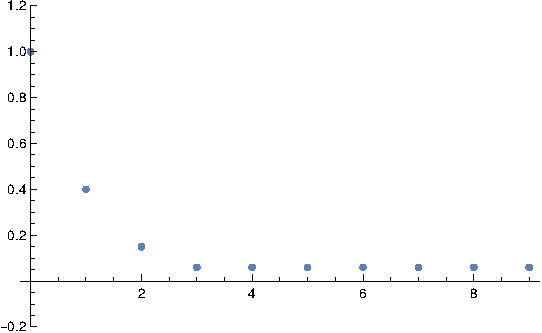
\includegraphics[width=0.32\linewidth]{analytics/images/exactCorrFns/lowDensLowL}  & 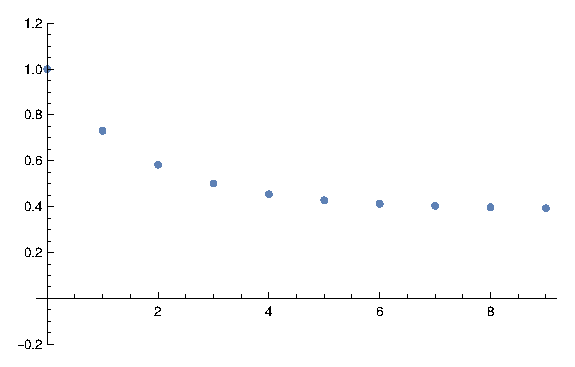
\includegraphics[width=0.32 \linewidth]{analytics/images/exactCorrFns/midDensLowL} & 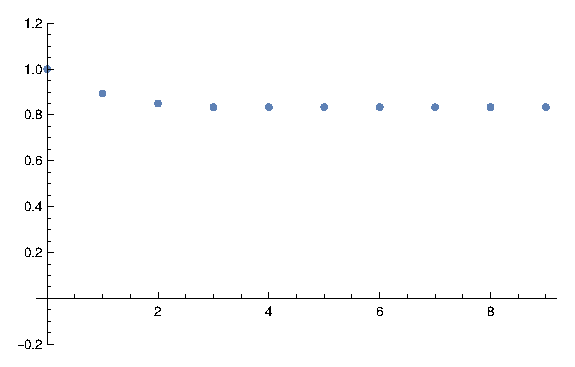
\includegraphics[width=0.32 \linewidth]{analytics/images/exactCorrFns/highDensLowL} \\
    \hline
    \raisebox{3 em}{ $1$ } & &    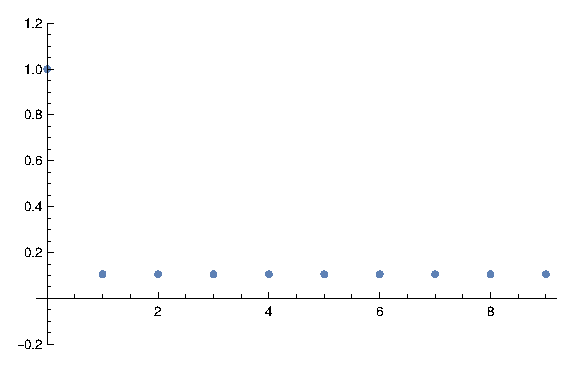
\includegraphics[width=0.32\linewidth]{analytics/images/exactCorrFns/lowDensMidL}  & 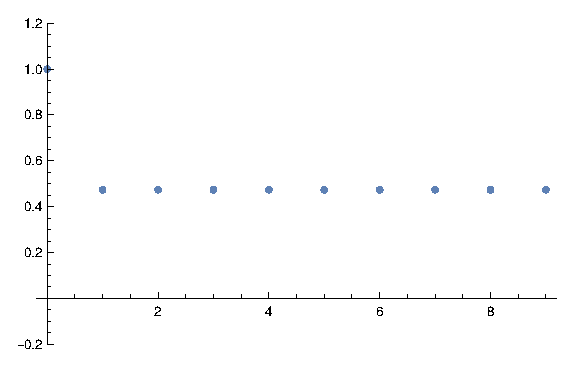
\includegraphics[width=0.32 \linewidth]{analytics/images/exactCorrFns/midDensMidL} & 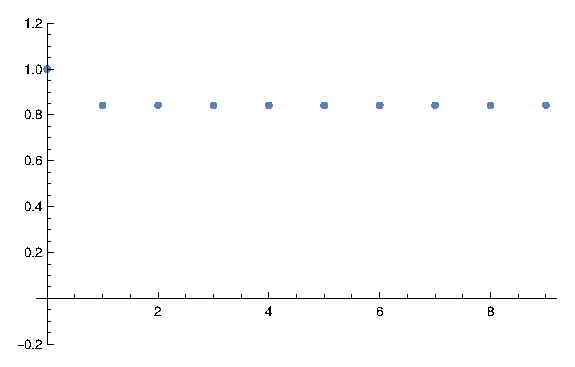
\includegraphics[width=0.32 \linewidth]{analytics/images/exactCorrFns/highDensMidL} \\
    \hline
    \raisebox{3 em}{ $10$ } & &    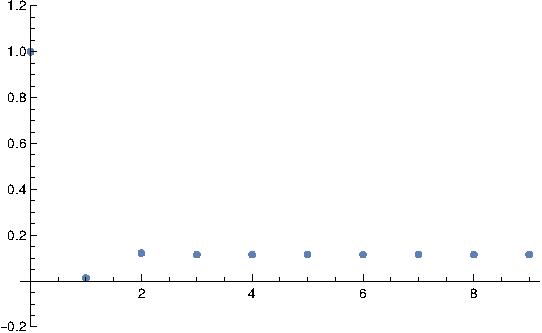
\includegraphics[width=0.32\linewidth]{analytics/images/exactCorrFns/lowDensHighL}  & 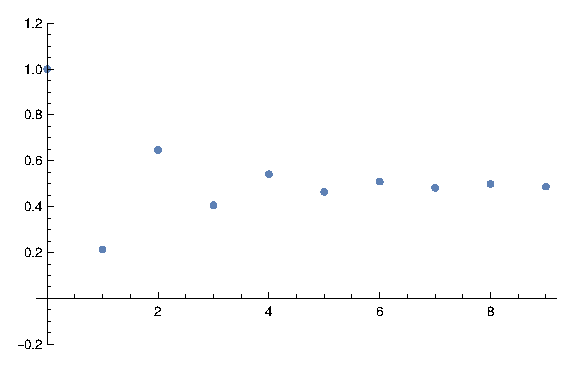
\includegraphics[width=0.32 \linewidth]{analytics/images/exactCorrFns/midDensHighL} & 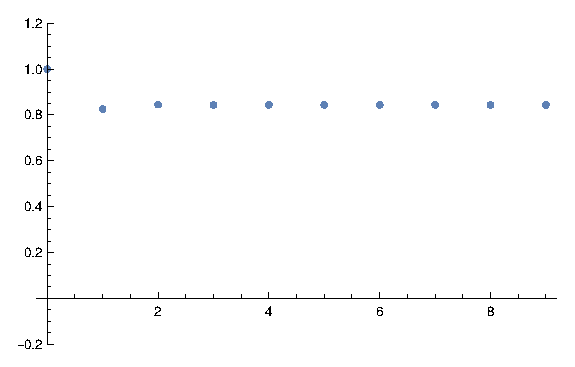
\includegraphics[width=0.32 \linewidth]{analytics/images/exactCorrFns/highDensHighL} \\
    \end{tabular}
\end{center}
    \vspace{-2em}
\end{figure}

Clearly, as $l$ becomes large, the correlation function tends to the density (note that the way we have define the correlation function it does not subtract this background probability; hence why many definitions do). Very small $\lambda$-values
cause particles to tend to cluster together, whilst large $lambda$ values cause particles and vacancies to tend to alternate. In theory we could use the equivalence with the Ising model to compute correlation lengths as a function
of $\rho$ and $\lambda$ by using the magnetic field in the original Ising model as a Lagrange multiplier in order to fix the total magnetisation (corresponding to particle number in the SPM). However, due to the fact that we cannot
accurately compute correlation functions to any decent accuracy using our numerics (see Chap.~\ref{}), we concluded that it was not worth the time to perform the calculation as we would have nothing to compare it to.

\subsection{Equivalence with the Misanthrope Process}

Keeping the SPM on a ring, there is a again a correspondence between it and the Misanthrope Process~\cite{evansWaclaw2014}. The Misanthrope Process is, like the SPM, defined by its rates. This time, however, there can be arbitrarily many particles
on a single lattice site. We can choose to consider the symmetric version, in which particles hop in either direction. The defining feature of the process is that particles hop from sites with occupation $m$ to adjacent sites with occupation
$n$ with some rate $u(m, n)$.

The equivalence between this and the SPM is made by identifying the \textbf{number} of particles on a site in the Misanthrope Process with the \textbf{length} of the gap between two particles in the SPM. In this way, one can see that a particle
moving, for example, one step right in the SPM corresponds to a particle moving from one stack to the adjacent one on the left in the Misanthrope Process. To complete the equivalence we set


\[
  u(m, n) =
  \begin{cases}
                                   \lambda, & n=0 \\
                                   1, & \text{otherwise.} 
  \end{cases}
\]

Using the result from~\cite{evansWaclaw2014}, that the probability weighting of a configuration $\{m_i\}$ may be factorised as
\begin{equation}
 P(\{m_i\}) \propto \prod_{i+1}^N f(m_i) \delta_{L+N, \sum_{j=1}^N m_j},
\end{equation}
where $f(m)$ is a weighting dependant on the occupation of a site,  we see that for the SPM $f(m) = \lambda^{-m}$. Thus, for finite $\lambda$ 
\begin{equation}
 \frac{f(m)}{f(m-1)} = \lambda^{-1}
\end{equation}
which remains bounded as $m \rightarrow \infty$, therefore this model does not exhibit explosive condensation, again by using~\cite{evansWaclaw2014}.

\subsection{Differences Between SEP and the SPM}

\section{Using the Mean-Field Approximation on the SPM}

For the reasons discussed above, we cannot analytically solve the SPM on a nonperiodic bounded domain in the same way as SEP. It could be the case that a complete analytic solution method exists, but if it does, we do not know of it, so
we will proceed on the assumption that the model is not analytically solvable. Therefore, it would be useful to at least possess approximate solutions, as this can help us by giving us something to test
our numerics against, and point us in the direction of interesting behaviours which might occur. We will start by deriving the MFT on a lattice, and will then take the continuum limit (as the lattice spacing tends to zero
relative to our scale of interest), as that should predict the dominant behaviour on the macroscopic scale.


\subsection{Lattice MFT Derivation}

As usual, in an MFT approximation, we will be saying that the equal-time probability of the $(i+1)^\mathrm{th}$ site being occupied is independent of the probability that the $i\mathrm{th}$ site is occupied.
More formally, let us denote the mean occupation of the $i^\mathrm{th}$ site at time $t$ by $\rho_i (t)$. When we invoke the mean-field approximation, we say that the mean occupations of sites at equal times are independent; thus,
the probability that site $j \ne i$ occupied given that site $i$ is occupied is $\rho_j (t)$. We can use this to calculate the rate at which $\rho_i (t)$ increases and decreases, and so obtain a system of coupled ODEs for $\rho_i (t)$.

Let us first consider the situation where the $i^\mathrm{th}$ site is unoccupied. The probability of this being the case is $(1-\rho_i (t))$. A particle could move from site $(i-1)$ or site $(i+1)$, but only if those sites are currently occupied.
Assuming that site $(i-1)$ is occupied (occurring with probability $\rho_{i-1}$ in MFT), the rate at which it would jump to site $i$ would depend on the occupation of site $(i-2)$,
as it would be $1$ if it was unoccupied and $\lambda$ if it was occupied. Phrasing this in MFT terms,
and suppressing $t$-dependence for brevity, the rate at which $\rho_i (t)$ is increased by particles coming from the left is
\begin{equation}
{\tau_0}^{-1} \left(1-\rho_i \right) \rho_{i-1} \left[ \left(1-\rho_{i-2} \right) \cdot 1  +   \rho_{i-2} \cdot \lambda \right].
\end{equation}
By symmetry, the income of particles from the right is
\begin{equation}
{\tau_0}^{-1} \left(1-\rho_i \right) \rho_{i+1} \left[ \left(1-\rho_{i+2} \right) \cdot 1  +   \rho_{i+2} \cdot \lambda \right].
\end{equation}
Using similar logic, but shifting things around slightly, the rate at which particles leave site $i$ to go to site $i+1$ is
\begin{equation}
{\tau_0}^{-1} \left(1-\rho_{i+1} \right) \rho_{i} \left[ \left(1-\rho_{i-1} \right) \cdot 1  +   \rho_{i-1} \cdot \lambda \right],
\end{equation}
and similarly 
\begin{equation}
{\tau_0}^{-1} \left(1-\rho_{i-1} \right) \rho_{i} \left[ \left(1-\rho_{i+1} \right) \cdot 1  +   \rho_{i+1} \cdot \lambda \right]
\end{equation}
is the rate at which particles leave $i$ to go to $i-1$.

At this point it becomes fairly clear why we introduced the quantity $\zeta = 1-\lambda$, as it neatens things up in general. The total rate at which particles enter site $i$ is
\begin{equation}
 {\tau_0}^{-1} \left(1-\rho_i \right) \left[ \left(1-\zeta \rho_{i-2} \right) \rho_{i-1} + \left(1-\zeta \rho_{i+2} \right) \rho_{i+1} \right]
\end{equation}
whilst they leave at rate
\begin{equation}
 {\tau_0}^{-1} \rho_i \left[ \left(1-\zeta \rho_{i+1} \right) \left(1 - \rho_{i-1} \right) + \left(1-\zeta \rho_{i-1} \right) \left(1 - \rho_{i+1} \right) \right]
\end{equation}
Combining the rates of arriving and leaving, we obtain our main result:
\begin{align}
\label{eq:latticeMFT}
\begin{split}
 \tau_0 \partDeriv{\rho_i}{t} &= \left( 1-\rho_i \right) \left[ \left(1-\zeta\rho_{i-2} \right) \rho_{i-1} + \left(1-\zeta\rho_{i+2} \right) \rho_{i+1} \right] \\
 &- \rho_i \left[ 2 \zeta \rho_{i-1} \rho_{i+1}  - (3-\zeta)\left(\rho_{i-1} + \rho_{i+1}\right) + 2 \right].
 \end{split}
 \end{align}
This is a nice result, and in theory we could stop right here and we could make a computational scheme for solving this as a sequence. However, there are a few issues. For one thing, $\rho_i (t)$ isn't the mean of a quantity
whose variance is being suppressed by the law of large numbers, as is desired when using the MFT approximation.
Thus, it is merely a rough sketch of what might happen, as variances and correlations between sites aren't suppressed. On the other hand, it simply relates the occupations of nearby sites,
whereas we would find a description of the bulk flow to be much more useful. Therefore, we may as well take the continuum limit to see how flow depends on concentration gradient and local density.

\subsection{Continuum Limit MFT Derivation}

To take the continuum limit, let's promote $\rho_i (t)$ to $\rho(x, t)$ so that 
\begin{equation}
\rho_{i+m}(t)~\rightarrow~\rho(x+am,t).
\end{equation}
Now we can Taylor expand for $\rho_{i+m} (t)$, as
\begin{equation}
 \rho(x+am,t) = \rho(x, t) + ma \partDeriv{\rho(x, t)}{x} + \frac{1}{2} m^2 a^2 \partDeriv{^2\rho(x, t)}{x^2} + \mathcal{O}(a^3). 
\end{equation}
Preferably with the aid of a computational algebra package (in my case \texttt{Wolfram Mathematica}), one may directly substitute Taylor expansions for the required $\rho_j$ into Eq.~\ref{eq:latticeMFT}, continuing to truncate
at $\mathcal{O}(a^3)$. Doing so, and collecting terms, we find that
\begin{align}
  \tau_0 \partDeriv{\rho}{t} =& a^2 \left[ 1-\zeta \rho (4-3\rho) \partDeriv{^2 \rho}{x^2}  \right]
  2 a^2 \zeta (3\rho-2) \left(\partDeriv{\rho}{x}\right)^2 + \mathcal{O}(a^4) ,
\end{align}
which may be factorised into the more convenient form
\begin{equation}
\label{eq:contPDE}
 \partDeriv{\rho}{t} = \frac{a^2}{\tau_0} \partDeriv{}{x} \left\{ \left[1 - \zeta \rho\left(4-3\rho\right) \right] \partDeriv{\rho}{x} \right\},
\end{equation}
which is a continuity equation
\begin{equation}
 \partDeriv{\rho}{t} = \partDeriv{J}{x} 
\end{equation}
with current
\begin{equation}
J = -\frac{a^2}{\tau_0} \left[1 - \zeta \rho\left(4-3\rho\right) \right] \partDeriv{\rho}{x}.
\end{equation}

Considering Fick's Law
\begin{equation}
 J = - D \partDeriv{\rho}{x},
\end{equation}
we see that our diffusion coefficient is
\begin{equation}
 D = \frac{a^2}{\tau_0} \left[1 - \zeta \rho\left(4-3\rho\right) \right].
\end{equation}
Setting $\zeta \rightarrow 0$ (i.e. $\lambda = 1$), we see that $D \rightarrow \frac{a^2}{\tau_0}$, which is consistent with what we would expect for the Symmetric Exclusion Process.

Clearly, the diffiusion coefficient varies quadratically with $\rho$. This is easiest to see via a few graphs, as shown in Fig.~\ref{fig:analDiffCoeffs}.
\begin{figure}[h!]
\caption{\label{fig:analDiffCoeffs} Plots of the variation of $\frac{a^2 D}{\tau_0}$ ($y$-axis) with respect to $\rho$ ($x$-axis), evalutated with various values of $\zeta$ (above plots).}
\begin{center}
 \begin{tabular}{c c}
     $\zeta = -0.15$ & $\zeta = 0$ \\ 
     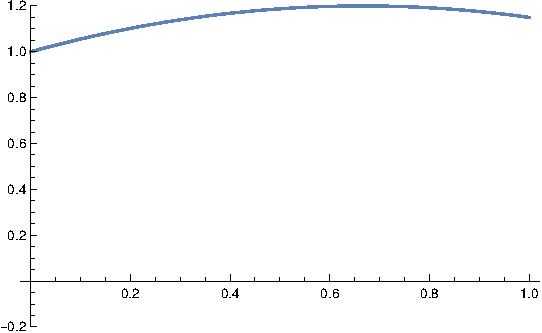
\includegraphics[width=0.49\linewidth]{analytics/images/diffCoeffs/diffCoeff-neg0-15}  & 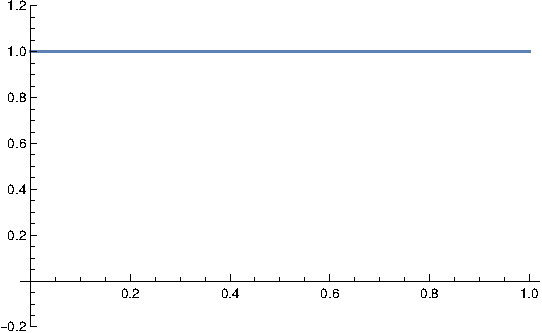
\includegraphics[width=0.49 \linewidth]{analytics/images/diffCoeffs/diffCoeff-0-0} \\
     $\zeta = 0.25$  & $\zeta = 0.5$ \\
     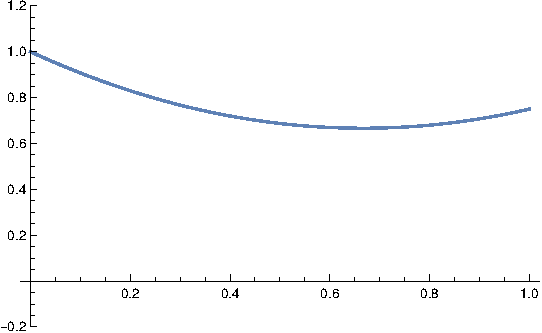
\includegraphics[width=0.49\linewidth]{analytics/images/diffCoeffs/diffCoeff-0-25}  & 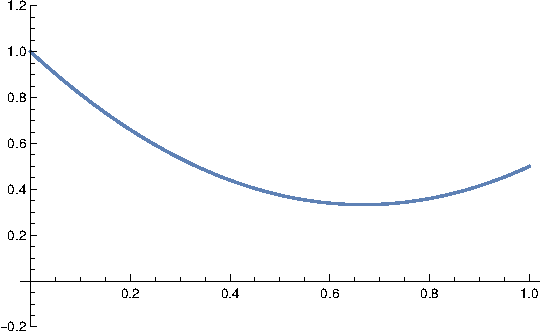
\includegraphics[width=0.49 \linewidth]{analytics/images/diffCoeffs/diffCoeff-0-5} \\
     $\zeta = 0.75$  & $\zeta = 0.9$ \\
     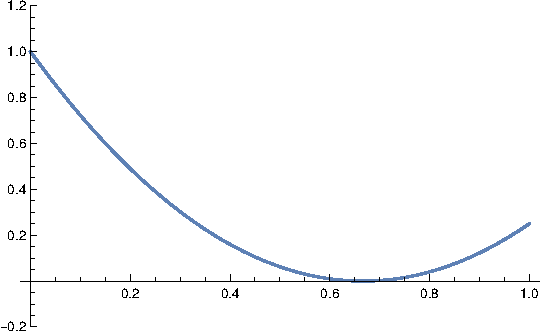
\includegraphics[width=0.49\linewidth]{analytics/images/diffCoeffs/diffCoeff-0-75}  & 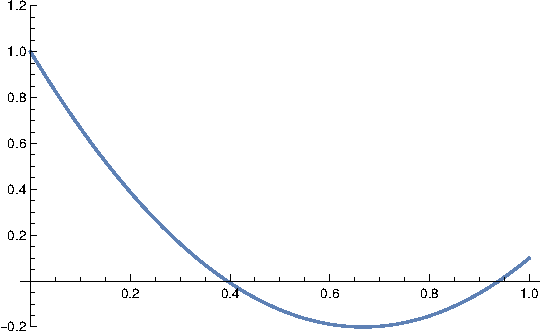
\includegraphics[width=0.49 \linewidth]{analytics/images/diffCoeffs/diffCoeff-0-9} \\
    \end{tabular}
\end{center}
    \vspace{-2em}
\end{figure}
Note that $D$ has a symmetry in $\rho$ around $\rho = \frac{2}{3}$, in the sense that $D$ is unchanged under $\rho \mapsto \frac{4}{3} - \rho$. Why this symmetry is present in the MFT is a little unclear ($\rho \mapsto 1 - \rho$
would be a much more obvious choice), however as you will see in the numerical simulations it does seem to be quite relevant, particularly in the high-$\lambda$ limit.

\subsection{Negative Diffusion Coefficients}
When do they happen? What do they mean?
\subsection{Continuum Limit MFT Solutions}
There's a bunch of these.
\subsection{Continuum MFT Breakdown}

\section{The SPM in Higher Dimensions}
Kinda repeat the earlier stuff in higher dimensions, particularly 2 where we actually have data. Maybe less need for elaborate sections structure here; just write freely and see how it goes.

